\usetikzlibrary{calc, positioning}
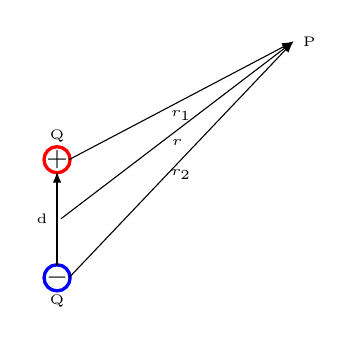
\begin{tikzpicture}[
        circ/.style = {circle, draw, minimum size =3mm, node contents={}}
    ]
    %Kreise
    \node (neg_pol)[circ, very thick, blue];
    \node at(0,0)[]{$-$};
    \node at(0,-0.1)[below]{\tiny{Q}};

    %Kreise
    \node at(0,1.5)(pos_pol)[circ, very thick, red];
    \node at(pos_pol.center)[]{$+$};
    \node at(0,1.6)[above]{\tiny{Q}};


    %Pfeile
    \draw[-latex] (0,0.15)      -- (0,1.35) node[left, midway]{\tiny{d}};
    \draw[-latex] (0.15,1.5)    -- (3,3) node[midway, below]{\tiny{$r_1$}};
    \draw[-latex] (0.05,0.75)   -- (3,3) node[right]{\tiny{P}} node[midway, below]{\tiny{$r$}};
    \draw[-latex] (0.15,0)      -- (3,3) node[midway, below]{\tiny{$r_2$}};


    %Legende

\end{tikzpicture}

